\section{Despliegue en entorno de pruebas}

El prototipo se despliega mediante Coolify \cite{coolify}, una plataforma de despliegue autoalojada que permite gestionar aplicaciones contenerizadas sobre infraestructura propia y construir la imagen de la aplicación directamente a partir del \textit{Dockerfile} del proyecto. Su elección responde a la necesidad de disponer de un mecanismo de despliegue reproducible y centralizado sobre el servidor utilizado para el entorno de pruebas, delegando en la plataforma tareas de infraestructura como el enrutamiento de solicitudes y la gestión de certificados TLS. La Figura \ref{fig:despliegue} presenta el diagrama de la infraestructura de despliegue.

La imagen del contenedor de aplicación se construye mediante un \textit{Dockerfile} multi-etapa con tres etapas diferenciadas. La primera etapa (\texttt{deps}) instala las dependencias del proyecto utilizando \texttt{pnpm} sobre una imagen base de Node.js 25 Alpine. La segunda etapa (\texttt{builder}) ejecuta la construcción de Next.js en modo \textit{standalone}\footnote{El modo \textit{standalone} de Next.js genera un servidor Node.js autocontenido que incluye únicamente las dependencias estrictamente necesarias para producción, sin requerir la carpeta \texttt{node\_modules} completa en el entorno de despliegue. Esto reduce significativamente el tamaño de la imagen Docker resultante.}, que produce un artefacto autocontenido con todas las dependencias necesarias para ejecutar el servidor en producción. La tercera etapa (\texttt{runner}) utiliza la imagen \texttt{node:25-bookworm-slim} e instala el intérprete de Racket como dependencia del sistema operativo mediante \texttt{apt-get}. Esta etapa copia únicamente el artefacto \textit{standalone}, el directorio de archivos estáticos y los tres archivos de instrumentación Racket, minimizando el tamaño de la imagen final. La variable de entorno \texttt{RACKET\_BIN} se configura en \texttt{/usr/bin/racket} para que la ruta de API localice el ejecutable sin depender de la configuración del sistema anfitrión.

El contenedor de la aplicación expone el puerto interno 3000, el cual no se publica directamente hacia el host. Coolify enruta las solicitudes externas hacia este puerto mediante un \textit{reverse proxy}\footnote{Coolify utiliza Traefik como \textit{reverse proxy} por defecto, encargado de dirigir las solicitudes entrantes hacia el contenedor correspondiente según el dominio configurado y de gestionar de forma automática los certificados TLS mediante Let's Encrypt \cite{coolify_traefik}.} que gestiona de forma automática, sin requerir la definición manual de reglas de enrutamiento en el proyecto. Esta arquitectura garantiza que el acceso externo al prototipo se realice exclusivamente a través del proxy, centralizando el control de las solicitudes entrantes.

\begin{figure}[H]
    \centering
    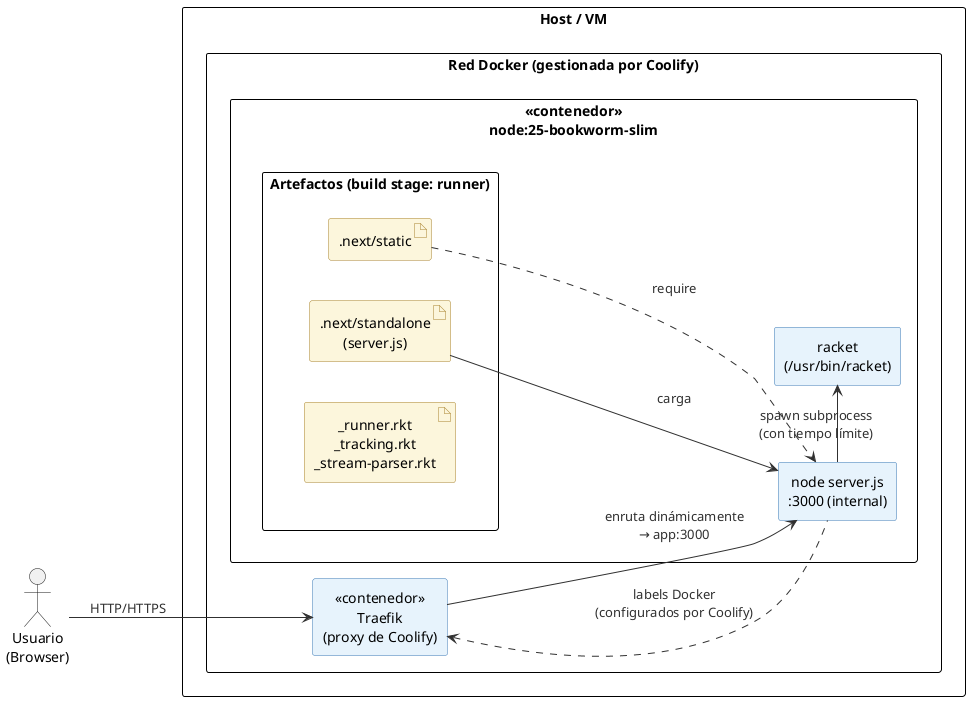
\includegraphics[width=0.85\textwidth]{Capitulo_5/imagenes/despliegue.png}
    \caption{Diagrama de despliegue del prototipo FLP Viewer en el entorno de pruebas}
    \scriptsize \textbf{Fuente:} Elaboración propia
    \label{fig:despliegue}
\end{figure}

\FloatBarrier
